\section{Theorie}

\subsection{Mikrowellen und Elektromagnetische Wellen }
Mikrowellen beschreiben elektromagnetische Wellen, die sich in einem vorher definierten Frequenzspektrum von 1 bis 300 $\si{\giga\hertz}$ befinden. 
Sie sind, im vergleich zu anderen alltäglichen Wellen, eher dem langwelligen Bereich zuzuordnen, weit jenseits dem für uns sichtbaren Lichts.
Elektromagnetische Wellen lassen sich hinreichend durch die Maxwell Glecihungen beschreiben, ohne jedoch dabei die Teilchen Eigenschaften der Korpuskeltheorie zu berücksichtigen. Im Folgenene Versuch wird sich außschließlich auf die Welleneigenschaften bezogen.
Charakteristisch für all diese Wellen ist die im Vakuum definierte Geschwindigkeit sich fortzubewegen, besser bekannt als Lichtgeschwindigkeit. Dort propagiert sie außschließlich als Transversalwelle.
Mit dieser Geschwindigkeit $c$, oder im Falle eines Mediums der entsprechend reduzierten, lässt sich nun die Wellenlänge mithilfe der Frequenz $\nu$ bestimmen.
\begin{equation}
    \label{eqn:1}
\lambda = c/{\nu}
\end{equation}
Das Magnetische Feld verhält sich analog zum elktrischen, steht aber zu jedem Zeitpunkt senkrecht auf seiner elktrischen Komponente. \\  Große Anwendug 
finden diese \enquote{Mikrowellen} unter anderem in der Funk - und Radartechnik. Zum Beispiel werden so durch abweichende Brechungsindexe und wechselnden Impedanzen,  Inforationen durch reflektierte Wellen gewonnen. 
Eine weitere Anwendung ist der Mikrowellenherd, der mit einer Charakteristischen Frequenz von $\SI{2.455}{\giga\hertz}$ die Dipole von Wassermoleküle passend ausrichtet, anregt und so Wärme erzeugt.

\subsection{Reflexklystron}

Das Reflexklystron ist ein Gerät um hochfrequentige Wellen entweder zu verstärken oder selbstständig anzuregen. Grundlage dazu sind zwei angeschlossene Spannungen, 
die zum einem die Resonatorkammer und zum anderen den wortgebenen Reflektor elektrisch laden. Zudem wird eine Glühkathode verwendet, die aus möglichen Metallen, 
gegen eine Austrittsarbeit, freie Elektronen löst und in Richtung des Reflektors beschleunigt. Wolfram bietet sich hierfür aufgrund der sehr hohen Schmelztemperatur sehr gut an.
Diese nun beschleuigten Elektroden finden ihren Weg zum Reflektor durch die Resonatorkammer und werden anschließend in diese Kammer zurückgelenkt. Die anfangs anegelegte Spannung treibt 
die Elektronen im Resonator folglich schwingend in die Richtung, die der negativen Spannungskomponente entgegengesetzt ist. Durch diese frequente Ausrichtung des Elektrischen Felds werden die emittierten Elektronen entweder weiter beschleunigt oder 
verlangsamt, was zu einer frequenzabhängigen Modulation der Geschwindigkeit führt. Während die Beschleunigung von Elektronen dem Resonator Energie kostet gewinnt er diese zurück, wenn Elektronen gebremst werden. 
Eine für den Resonator optimnale Laufzeit für Energiegewinnung ist 
\begin{equation}
    \left(n+ \frac{3}{4} \right) \cdot T  \quad \quad n \in \mathbb{N}_0.
\end{equation}
Die so entstehende Schwingung wird anschließend durch einen Hohlwellenleiter ausgekoppelt und weiter transportiert.
\begin{figure}
    \centering
    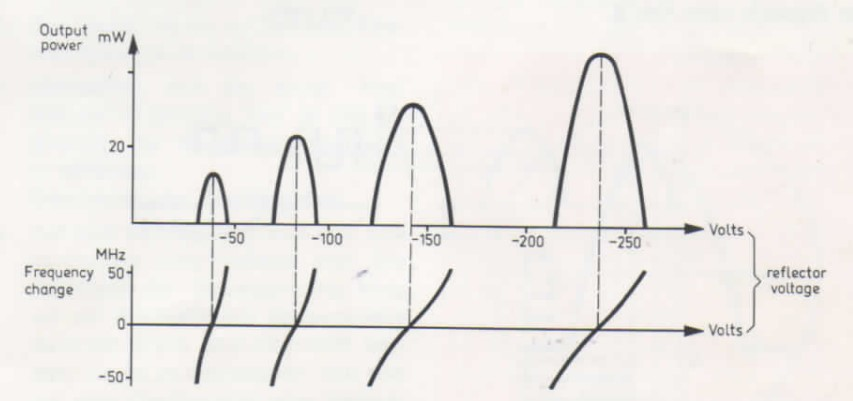
\includegraphics[width=0.8\textwidth]{bilder/dia.jpg}
    \caption{In Diesem Diagram ist die abgegriffene Leistug der Wellenmoden aus einem Reflexklystron, abhängig von der angelegten Reflektorspannung dargestellt.
    Die entsprechende Frequenz ist darunter mit gleicher Abszisse dargestellt. Deutlich erkennbar sind hier die einzelenen Moden die durch die Modulation entstehen.} 
    \label{fig:ref}
\end{figure}
\begin{figure}
    \centering
    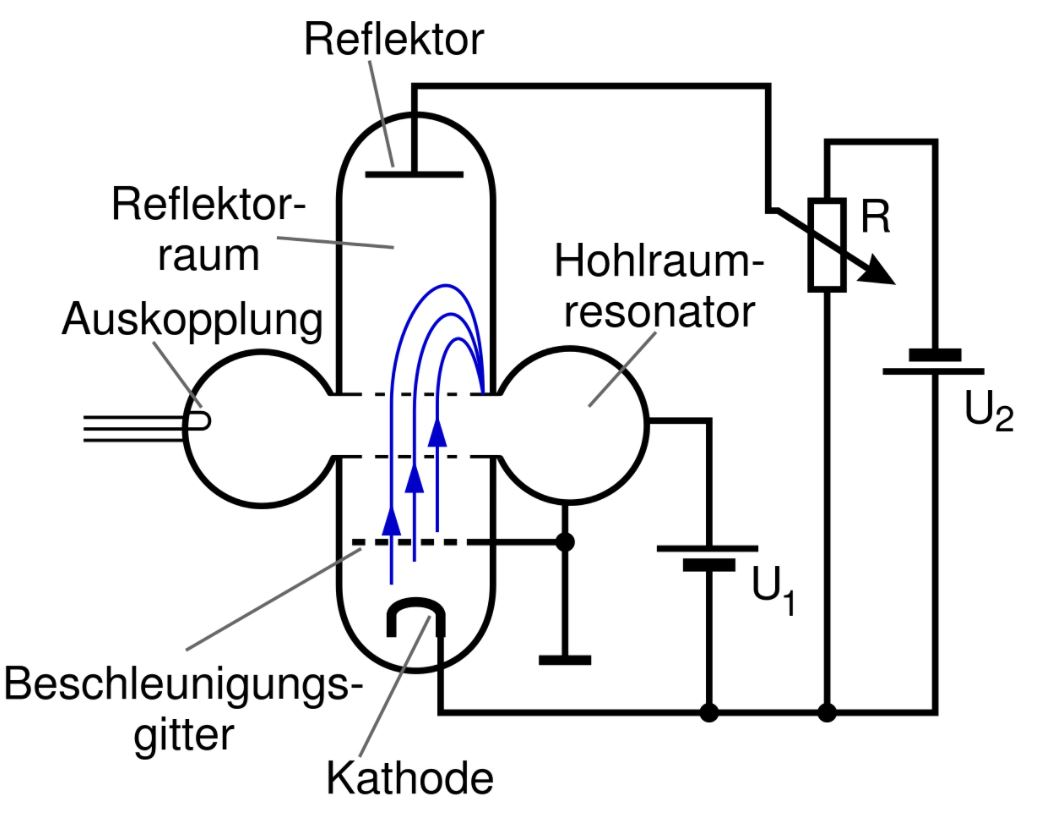
\includegraphics[width=0.6\textwidth]{bilder/theo.JPG}
    \caption{Schematischer Aufbau eines Reflexklystrons. Deutlich zu erkennen sind die blauen Pfeile, die verschiedene Elektronen abhängig von der angelegten Spannung darstellen. 
    Diese Sammlung an Elketronen nennt sich \enquote{Bunching}.} 
    \label{fig:ref}
\end{figure}
Durch Änderungen am internen Aufbau des Klystron lassen sich die Moden unteranderem durch Spannungsunterschiede verschieben. 
\begin{equation}
    P_{\text{Output}} (\si{\volt}) \sim P_{\text{Output}} (\si{\volt} + \tau)
\end{equation}
Die Variabel $\tau$ ist hier so gewählt, dass $\si{\volt} + \tau$ wieder die vorher von $\si{\volt}$ getroffene Mode beschreibt.
Analog lässt sich die Frequenz durch den mechanischen Aufbau ändern. Eine größere Resonatorkammer würder den Elektronen 
mehr Laufzeit bieten und so das \enquote{Bunching} verlangsamen.

\subsection{Hohlleiter}
Für die Fortleitung von elektromagnetischer Strahlung gibt es einige Methoden. Eine davon ist die Verwendung von Hohlleitern. Sie sind besonders gebräuchlich bei der Verwendung von Mikrowellen, also bei Frequenzen im $\si{\giga\hertz}$-Bereich.
Dies liegt vorallem daran, dass sie in diesem Bereich besonders verlustarm sind. Koaxialkabel stellen beispielsweise eine andere Möglichkeit dar, sie sind allerdings auf Grund der mit der Frequenz steigenden Absorption deutlich 
verlustanfälliger. Bei beiden Leitern wird, wie es der Name schon verrät, ein leitender Stoff an der Außenseite angebracht, an dem die elektromagnetische Welle reflektiert werden kann. Diese Reflexion kann in der Theorie ohne Randeffekte natürlich unendlich oft
wiederholt werden und würde so einen verlustfreien Leiter darstellen. Hohlleiter sind, wie zu erwarten innen hohl, also mit Luft gefüllt.
\\
\newline
Wie eine solche elektromagnetische Welle in einem Leiter propagiert hängt vollständig von den vorliegenden Randbedingungen ab. Mit diesen Randbedingunge lassen sich dann die Maxwellgleichungen für das elektrische, sowie das magnetische Feld lösen.
Die Form eines Hohlleiters ist beliebig für die Applikation wählbar. Der gängigste und auch in diesem Versuch verwendete Hohlleiter, ist ein Rechteckhohlleiter. 
\\
\newline
Zunächst einige Überlegungen zu den Randbedingungen an einem Rechteckhohlleiter. Die ummantelnde Fläche des Hohlleiters kann als nahezu perfekt leitend angenommen werden. In der Regel wird dazu Kupfer oder Aluminium verwendet. Diese bildet eine 
Äquipotentialfläche, also muss die parallele Komponente des E-Feldes an jedem Rand des Leiters verschwinden. Daraus folgt, dass die Rotation des E-Feldes dort ebenfalls verschwindet und somit die tangentiale Komponente des B-Felder ebenfalls
verschwinden muss. Die Bedingungen lauten also
\begin{align*}
E_{||} &= 0, \\
B_{⊥} &= 0.
\end{align*}
Wenn nun also der Querschnitt eines Hohlleiters betrachtet wird, müssen diese Randbedinungen in jede einsichtbare Raumrichtung erfüllt sein. Daraus folgt unteranderem das die typische transversale Form von EM-Wellen im Vakuum nicht mehr vorliegen kann, denn
die E, und B-Komponente müssen senkrecht aufeinander stehen, allerdings sind die nötigen Freiheitsgrade nicht mehr gegeben, um auch senkrecht zur Ausbreitungsrichtung zu stehen. In einem Rechteckhohlleiter ist also eine Komponente immer
longitudinal. Beschrieben werden die Wellen durch verschiedene Moden, denn durch die Reflektion an den Wänden bilden sich stehende Wellen, die nun je nach Frequenz unterschiedlich viele Schwingungsbäuche ausbilden. 
\\
\newline
Gekennzeichnet werden die einzelnen Moden in Rechteckhohlleitern durch $\textbf{TE}_{m,n}$ oder $\textbf{TM}_{m,n}$. Dabei steht die $\textbf{TE}$ für transversal elektrisch mit dementsprechend longitudinaler B-Komponente und $\textbf{TM}$ genau umgekehrt. Der Fall $\textbf{TEM}_{m,n}$ wurde
bereits wie vorher erklärt ausgeschlossen. Die Zahlen $m$ und $n$ geben dabei die Mode an und sie können jede beliebige natürliche Zahl, sowie auch Null, annehmen. Sie beschreiben wie viele Wellenbäuche der stehenden Welle in beispielsweise $x$, und $y$-Richtung passen.
Genauer gesagt stellen sie eine Bedingung der jeweiligen Wellenzahl in dessen Raumrichtung auf. Typischerweise werden in Hohlleitern Frequenzen verwendet, bei denen sich $\textbf{TE}_{1,0}$ oder $\textbf{TM}_{1,0}$ Wellen ausbilden. In der Abbildung \ref{fig:4} ist eine 
schematische Skizze einer solchen Mode dargestellt.

\begin{figure}
    \centering
    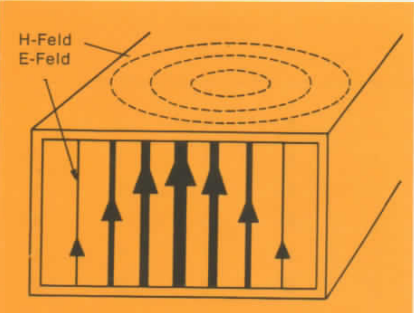
\includegraphics[width=0.4\textwidth]{bilder/mode.png}
    \caption{Darstellung einer $\textbf{TE}_{1,0}$-Mode in einem Rechteckhohlleiter. \cite{skript}} 
    \label{fig:4}
\end{figure}
Durch die zuvor erwähnten Randbedingungen zeigt sich jetzt allerdings auch, dass es eine Grenzwellenlänge gibt, unter der keine Welle innerhalb des Leiters mehr propagieren kann. Formal ergibt sich diese durch die Existenz einer reellen Wellenzahl 
in Ausbreitungsrichtung. 
Die Grenzwellenlänge eines Rechteckhohlleiters einer beliebigen Mode lautet
\begin{equation}
\lambda_{g} = \frac{2}{\sqrt{\left(\frac{m}{a}\right)^2 + \left(\frac{n}{b}\right)^2}}.
\end{equation}
Für den typischen $\textbf{TE}_{1,0}$-Modus ergibt dies 
\begin{equation}
    \lambda_{g} = 2a,
\end{equation}
was ebenfalls geomeetrisch einsichtbar ist.
\\
Die longitudinale Komponente erfährt ebenfalls eine zur im freien Raum verschobene Wellenlänge, welche durch
\begin{equation}
    \lambda_{h} = \frac{\lambda_0}{\sqrt{1 - \left(\frac{\lambda_0}{\lambda_{g}}\right)^2}}.
\end{equation}
berechnet wird. Dabei gibt $\lambda_0$ die Wellenlänge im freien Raum an. Aus der klassischen Beziehung \ref{eqn:1} lässt sich nach leichter Umformung auch die Frequenz in Ausbreitungsrichtung als
\begin{equation}
    \label{eqn:222}
    f = c \cdot \sqrt{\left(\frac{1}{\lambda_h}\right)^2 - \left(\frac{1}{2a}\right)^2}
\end{equation}
angeben.


\subsection{Stehwellenverhältnis} 
Häufig, durch Reflexion von Hindernissen oder anderen Faktoren, treten Wellen als sogenannte \enquote{stehende Wellen} auf. Das charakteristische Merkmal sind die nicht verschobenen Nullpunkte bei einer varibler Zeit $t$.
Bei Reflexion erfährt die rücklaufende Welle einen Phasensprung und formt so durch Superposition mit der einfallenden Welle eine Überlagerung. Die ursprüngliche Welle wird so periodisch verstärkt, abgeschwächt oder ganz annuliert. 
In der Anwendung treten solche Reflexionen vorallem durch Impedanzunterschiede oder materielle Störungen auf. Die daraus folgene Proportionalität zwischen dem der Reflexionsamplitude $I_{ref}$ und einem etwaigen Impedanzunterschiede $\Delta Z$
führt zu einer Definition des \enquote{Stehwellenverhältnis} SWR. (SWR für \enquote{Standing Wave Ratio}) 
\begin{equation*}
    I_{ref} \sim \Delta Z \sim \text{SWR macht eig kein sinn da sreinzunehmen oder?}.
\end{equation*}
Dieses Verhätnis beschreibt die Überlagerung der Wellen, also der resultierenden Amplitude, bei ihrer maximalen -und ihre minimalen Auslenkung. 
Gemessen werden die Amplituden bei elektrischen Leitern meist direkt durch das elektrische Feld $E$ oder der Spannung $U$, da diese proportional zueinander sind.
Alternativ lassen sich die einzelnen Komponenten, die zu Superposition führen, getrennt betrachten. Hier entsteht das Verhältnis aus der maximal moöglichen, verstärkten Amplitude $|E_i| + |E_r|$ und dem abschgeschwächten Anteil$|E_i| - |E_r|$.
Der Betrag der einfallenden Feldstärke ist als $E_i$ -und der reflektierte als $E_r$ gekennzeichnet. Dieses eignet sich also gut zur Quantisierung der Güte eines entsprechend leitenden Mediums. Bei einem Verhältnis von $1$ wäre die Leitung perfekt.
\begin{equation}
    \text{SWR} = \frac{E_{max}}{E_{min}} =  \frac{|E_i| + |E_r|}{|E_i| - |E_r|}
\end{equation}
Eine äquivalente Beschreibung ist durch die sogenannte \enquote{Dämpfung} möglich. Diese hat die abolute Einheit $\si{\decibel}$ und beschreibt das Verhältnis von optimaler -und, durch z.B. Reflexion, abgeschwächter Leistung $P$. 
\begin{equation}
    \si{\decibel} = 10 \cdot \text{log} \frac{P_1}{P_2}
\end{equation}
Auffallend ist, dass wenn das Verhältnis aus den Leistungen $P_1$ und $P_2$ eben genau $2$ ergbit, eine Dämpfung von 3 $\si{\decibel}$ folgt
\begin{equation*}
    \si{\decibel} = 10 \cdot \text{log} 2 = 3.
\end{equation*}
Dieser Zusammenhang kann durch 
\begin{equation}
    \text{SWR} =\sqrt{1 + \frac{1}{ sin^2 \left( \frac{\pi (d_1 - d_2)}{\lambda_h}  \right)} } 
\end{equation}
zum Stehwellenverhältnis führen, da die Leistung eng mit der elektrischen Spannung verknüpft ist. 
Hier ist $\lambda_h$ die Wellenlänge im Hohlleiter und $d_1$ und $d_2$ sind die Abstände von einem gewählten Minimum, so dass sich die Leistung verdoppelt wird. \\
Alternativ können mit der \enquote{Abschwächer-Methode} und zwei $\si{\decibel}$ Werten das Verhältnis errechnet werden.
\begin{equation}
    \text{SWR} = 10^{\frac{A_2-A_1}{20}}
\end{equation}
